% Appendix A

\chapter{Installation of 4DIAC-IDE} % Main appendix title

\label{AppendixA} % For referencing this appendix elsewhere, use \ref{AppendixA}

\section{4DIAC IDE installation}

The installation of 4DIAC-IDE is independent from the used operating system. In order to run 4DIAC-IDE you require Java 1.7 SDK or later, whereas it is currently NOT recommended to use Java 8.

To install 4DIAC-IDE you simply download the latest version for your operating system from https://eclipse.org/4diac/. Unzip it to any desired folder and start the 4DIAC-IDE. It already contains a function block library, some sample applications and also pre-build versions of FORTE. If you only want to use available Function Blocks you are ready to go.

\textbf{Building your own 4DIAC-IDE from source:} Running 4DIAC-IDE from source has the great advantage that you can easily keep up with the developments performed in the Mercurial repository. In case you want to run 4DIAC-IDE from source follow the Installation steps at https://eclipse.org/4diac/documentation/help.html
%----------------------------------------------------------------------------------------
%	SECTION 2
%----------------------------------------------------------------------------------------

\section{FORTE compilation}

For conducting first experiments with 4DIAC you can use the pre-build version of FORTE which comes along in the runtimes directory of the 4DIAC-IDE package. However if you want to develop your own Function Blocks or you want to run FORTE on different control devices you have to download and build FORTE from source.

The compiling and debugging of FORTE consists of few steps:

\textbf{Download source code}
You can download the latest Version of FORTE on http://www.eclipse.org/4diac/. Extract the file into your desired working directory.
You can also use Mercurial Hg like TortoiseHG to get FORTE from http://hg.code.sf.net/p/fordiac/forte.

\textbf{Prepare compilation and linking tools
}In case you want to create own function blocks, or edit existing one you are going to compile your own version of FORTE. According to your operating system, you have several options to choose. 
In Linux – like systems required packages to compile are:
\begin{itemize}
	\item binutils 
	\item gcc 
	\item gdb
	\item make
\end{itemize}
In case you are Mac user you can compile FORTE in X-Code. 
Compiling on Windows is most complicated. There are few possibilities:
\begin{itemize}
	\item Compiling and Debbugging FORTE with MS Visual Studio Express
	\item Compiling using Cygwin 
	\item Compiling using MinGW – I have used this option. Whole subsection is dedicated to this option
\end{itemize}

\textbf{CMake for generating the make file}

CMake helps you to configure FORTE for compilation with your desired development environment or hardware device. For starters we recommend to use the GUI tool that comes with CMake.

When starting the CMake-GUI you have to select the source directory, which is the main FORTE directory and the bin directory (e.g.FORTE/bin/posix) which is the output directory. There CMake will put the build project files (e.g., the makefiles) as well as any configuration data. 


\begin{figure}
\centering
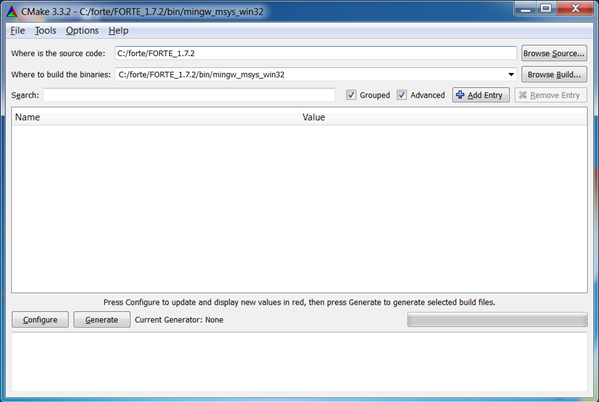
\includegraphics{Figures/cmake-1}
\decoRule
\caption[CMake step 1]{Selection of source data and output folder}
\label{fig:cmake-1}
\end{figure}
 
After that you will need to press the configuration button. A window will pop up that lets you select the kind of project you like to build. In this step you have to have installed compillers. 
Select MSYS Makefiles as the generator for this project.

\begin{figure}
\centering
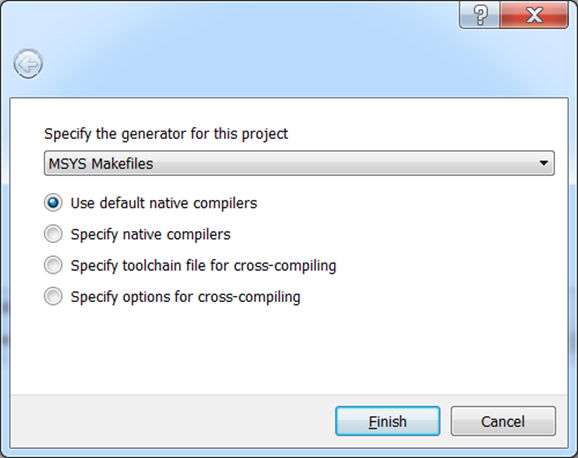
\includegraphics{Figures/cmake-2}
\decoRule
\caption[CMake step 2]{Specifing the generator}
\label{fig:cmake-2}
\end{figure}
 

For the correct Project Setting please have a look at the next step. In the CMake main window a list of red marked options will appear. These options allow you to configure your FORTE build. The minimal configuration you have to perform is to select the architecture you like to build for (e.g., FORTE\_ARCHITECTURE to POSIX / WIN32) and the modules with the function block libraries you like to use. You should also keep FORTE\_SUPPORT\_MONITORING enabled for Debugging and FB-Testing.

\begin{figure}
\centering
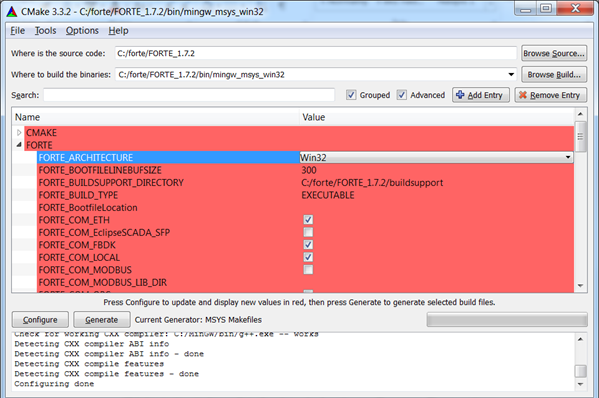
\includegraphics{Figures/cmake-3}
\decoRule
\caption[CMake step 3]{Configuring architecture of compilled FORTE}
\label{fig:cmake-3}
\end{figure}
 

Then you need to press again the configure button and depending on your selection in the previous step new options (marked in red) may appear. Press configure until no new options are appearing and then the generate button for generating the project files.

\begin{figure}
\centering
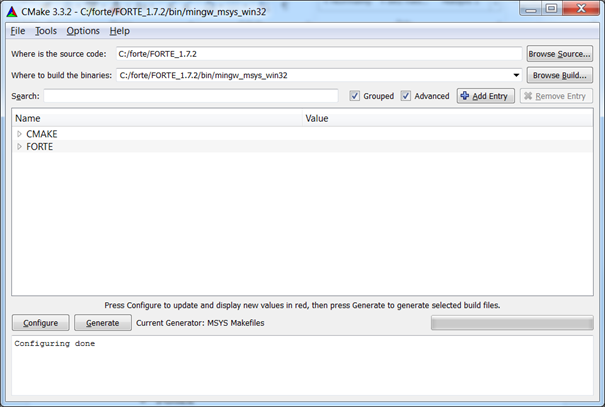
\includegraphics{Figures/cmake-4}
\decoRule
\caption[CMake step 4]{Configuration done.}
\label{fig:cmake-4}
\end{figure}
 
After that you can start the build process.

Configuration of CMake for different OS:
\begin{table*}
	\centering
		\begin{tabular}{c | c}
			\textbf{Windows} & \textbf{POSIX} \\
			FORTE\_ARCHITECTURE\_WIN32  & FORTE\_ARCHITECTURE\_POSIX \\
			FORTE\_MODULE\_CONVERT & FORTE\_MODULE\_CONVERT \\
			FORTE\_MODULE\_IEC61131 & FORTE\_MODULE\_IEC61131 \\
			FORTE\_MODULE\_OPC\_UA & FORTE\_MODULE\_OPC\_UA \\
			FORTE\_MODULE\_Test & FORTE\_MODULE\_Test \\
			FORTE\_MODULE\_UTILS & FORTE\_MODULE\_UTILS \\
			FORTE\_SUPPORT\_MONITORING & FORTE\_SUPPORT\_MONITORING \\
 
		\end{tabular}
\end{table*}


\textbf{IDE to work with the FORTE code}
You can use different development Environments, whereas the C++ Compiler you can use to build FORTE not only depends on this environment but also on your operating system. For compiling FORTE under Windows you can use either Visual Studio (Express or full edition) or Eclipse. When using Eclipse for development and debugging under Windows you will need to use a Posix emulation environment like cygwin or minGW.
\begin{itemize}
	\item Compiling and Debugging FORTE with MS Visual Studio Express
	\item Compiling and Debugging FORTE with Eclipse
	\item Compiling and Debugging FORTE with CodeBlocks
\end{itemize}

For the development with FORTE the understanding of the general file structure is helpful. Therefore the essential parts as well as the Makefiles which are important for the configuration and compilation of FORTE are listed in the following:
\begin{itemize}
	\item \textsl{src/modules} this folder contains the source code (cpp, h) of all Function Blocks available for FORTE
	\item \textsl{bin/<yourSystem>/src} contains the forte executable after compilation with Makefile all
	\item \textsl{bin/<yourSystem>/src\_gen} contains the object files generated during compilation with Makefile all
	\item all this Makefile generates the object files for all FORTE core files and Function Block source code files
	\item clean this makefile removes all generated object files.
\end{itemize}


\section{Installing and Settipg up MinGW for FORTE Development}

Download and install MinGW from http://www.mingw.org/
Launch MinGW installer and install default setting and add following packages:

\begin{itemize}
	\item Mingw32-gcc
	\item Mingw32-gcc-g++
	\item mingw32-make
	\item msys-make 
	\item mingw32-libz ( newer version of windows doesn’t include libraries)
	\item mingw32-gmp ( newer version of windows doesn’t include libraries)	
\end{itemize}


After install go to the Control Panel/System/Advanced/Environment Variables.  Change PATH variable (click on it) add path where your MinGW binaries have been installed in e.g., C:\\MinGW\\bin\\;. Add C:\\MinGW\\bin;C:\\MinGW\\msys\\1.0\\bin; in the Windows file PATH. 
\textbf{Test MinGW}
Open command prompt window by pressing Windows button and entering cmd. Enter bash, if bash prompt appears it was successful.
